\chapter{Anotační rozhraní}
\label{chap:rozhrani}

V rámci této práce bylo implementováno anotační rozhraní pro~vyhodnocování algoritmů, které přiřazují vhodné obrázky k~textům. Anotační rozhraní je velmi univerzální. Anotátor má ve~webové aplikaci v~levém sloupci novinový text a v~pravém sloupci galerii obrázků. Jeho úkolem je označit obrázky, které se k~danému textu hodí, a obrázky, které se k~textu nehodí. Má také možnost nechat obrázek neoznačený, pokud by se nemohl rozhodnout ani pro~jednu variantu.

\section{Instalace rozhraní}

Celé rozhraní je aplikace napsaná v~jazyce Ruby a frameworku Ruby on Rails. Aplikace je volně šiřitelná pod licencí MIT. pro~zprovoznění anotační aplikace je potřeba UNIXový systém (Linux, Mac). Zdrojový kód aplikace je uložen na~severu GitHub\footnote{\url{https://github.com/hypertornado/cemi_anotace}} a nejlépe lze stáhnout pomocí gitu. pro~běh serveru je potřeba verze ruby 2.0 a vyšší. Celá aplikace se zprovozní následujícím pořadím BASH příkazů:

\begin{lstlisting}[language=bash]
git clone https://github.com/hypertornado/cemi_anotace
cd cemi_anotace
bundle install #nainstaluje vsechny ruby zavislosti
rake db:migrate #vytvori sqlite databazi s tabulkami
rails server #spusti anotacni server na portu :3000
\end{lstlisting}

\section{Přidání uživatelů}

Po spuštění serveru je možné přidat anotátory \href{http://localhost:3000/users}{v administračním rozhraní}. Přístup je zaheslován HTTP autentifikací. Defaultní uživatelské jméno je cfo a heslo cfo85. Administrátorské přístupové údaje lze změnit v~souboru\\\lstinline{ROOT_APLIKACE/app/controllers/admin_controller.rb}. Uživatelé mají pouze dvě datové položky --- uživatelské jméno (Name) a heslo (Password). Uživatele lze přidávat, mazat a upravovat. Nepředpokládá se, že by anotovaná data byla vysoce citlivá, heslo je proto v~databázi uloženo v~plaintextu.

\section{Import anotačních dat}

Data pro~anotaci lze nahrát pomocí příkazu

\begin{lstlisting}[language=bash]
rake data:import
\end{lstlisting}

Příkaz očekává existenci souboru\\\lstinline{ROOT_APLIKACE/public/annotation_inputs.csv}. Ten musí mít speciální formát, kdy je každý řádek rozdělen mezerami na šest sloupců s následujícími položkami:

\begin{description}

\item[INDEX] \hfill \\
  unikátní číslo jedné anotace.
\item[LABEL] \hfill \\
 interní popis pokusu.
\item[PRIORITY] \hfill \\
 priorita, celé číslo $>= 0$. Určuje prioritu s jakou se má anotace přiřadit. Čím vyšší číslo, tím vyšší priorita.

\item[PREFER\_USER] \hfill \\
 uživatelské jméno preferovaného anotátora. Pokud není žádný anotátor preferován, použije se pomlčka.
\item[TEXT\_FILE] \hfill \\
 cesta k~textovému souboru s referenčním článkem.
\item[IMAGE\_FILES] \hfill \\
 seznam cest k~obrázkům. Cesty nemohou obsahovat mezery a jsou oddělené středníkem.
\end{description}

Ukázka importovaných dat:

\begin{lstlisting}[language=bash]
1 basics 0 - ./text/aha/aha-00263.txt.gz  img/1.jpg;img/2.jpg;img/3.jpg
2 basics 1 - ./text/aha/aha-00006.txt.gz  img/1.jpg;img/2.jpg
3 basics 0 - ./text/aha/aha-00009.txt.gz  img/2.jpg
\end{lstlisting}

\section{Export anotačních dat}

Hotové anotace lze exportovat příkazem

\begin{lstlisting}[language=bash]
rake data:export
\end{lstlisting}

Tento příkaz vypíše na konzolu řádky, které mají tabulátorem oddělené položky:

\begin{description}

\item[INDEX] \hfill \\
  ID anotace. Stejné jako u importovaných dat.
\item[USER] \hfill \\
  Jméno anotátora, který anotaci vytvořil.
\item[TIME] \hfill \\
  Čas uložení hotové anotace ve~formátu UNIX timestamp.
\item[SKIPPED] \hfill \\
  Pokud uživatel anotaci přeskočil, je hodnota True, jinak False.
\item[APPROPRIATE] \hfill \\
  Seznam obrázků které anotátor označil jako vhodné k~textu ve~formátu relativních cest oddělených středníkem.
\item[NOT\_APPROPRIATE] \hfill \\
  Seznam obrázků které anotátor označil jako nevhodné k~textu ve~formátu relativních cest oddělených středníkem.

\end{description}

\section{Import obrázků a textů}

Anotační texty a obrázky musí být nahrány do~adresáře \lstinline{ROOT_APLIKACE/public} tak, aby jejich cesty odpovídaly cestám v~souboru \\ \lstinline{ROOT_APLIKACE/public/annotation_inputs.csv}. Pokud tedy importovaný soubor obsahuje cestu k~obrázku \lstinline{img/1.jpg}, musí být nahrán odpovídající soubor do~\lstinline{ROOT_APLIKACE/public/img/1.jpg}.

Obrázky musí být ve~formátu, který podporují webové prohlížeče, tedy hlavně JPEG a PNG. Texty musí být uloženy v~textových souborech s kódováním utf-8 a komprimovaný pomocí gzip\footnote{\url{http://www.gzip.org/}}.

\begin{figure}
  \centering
  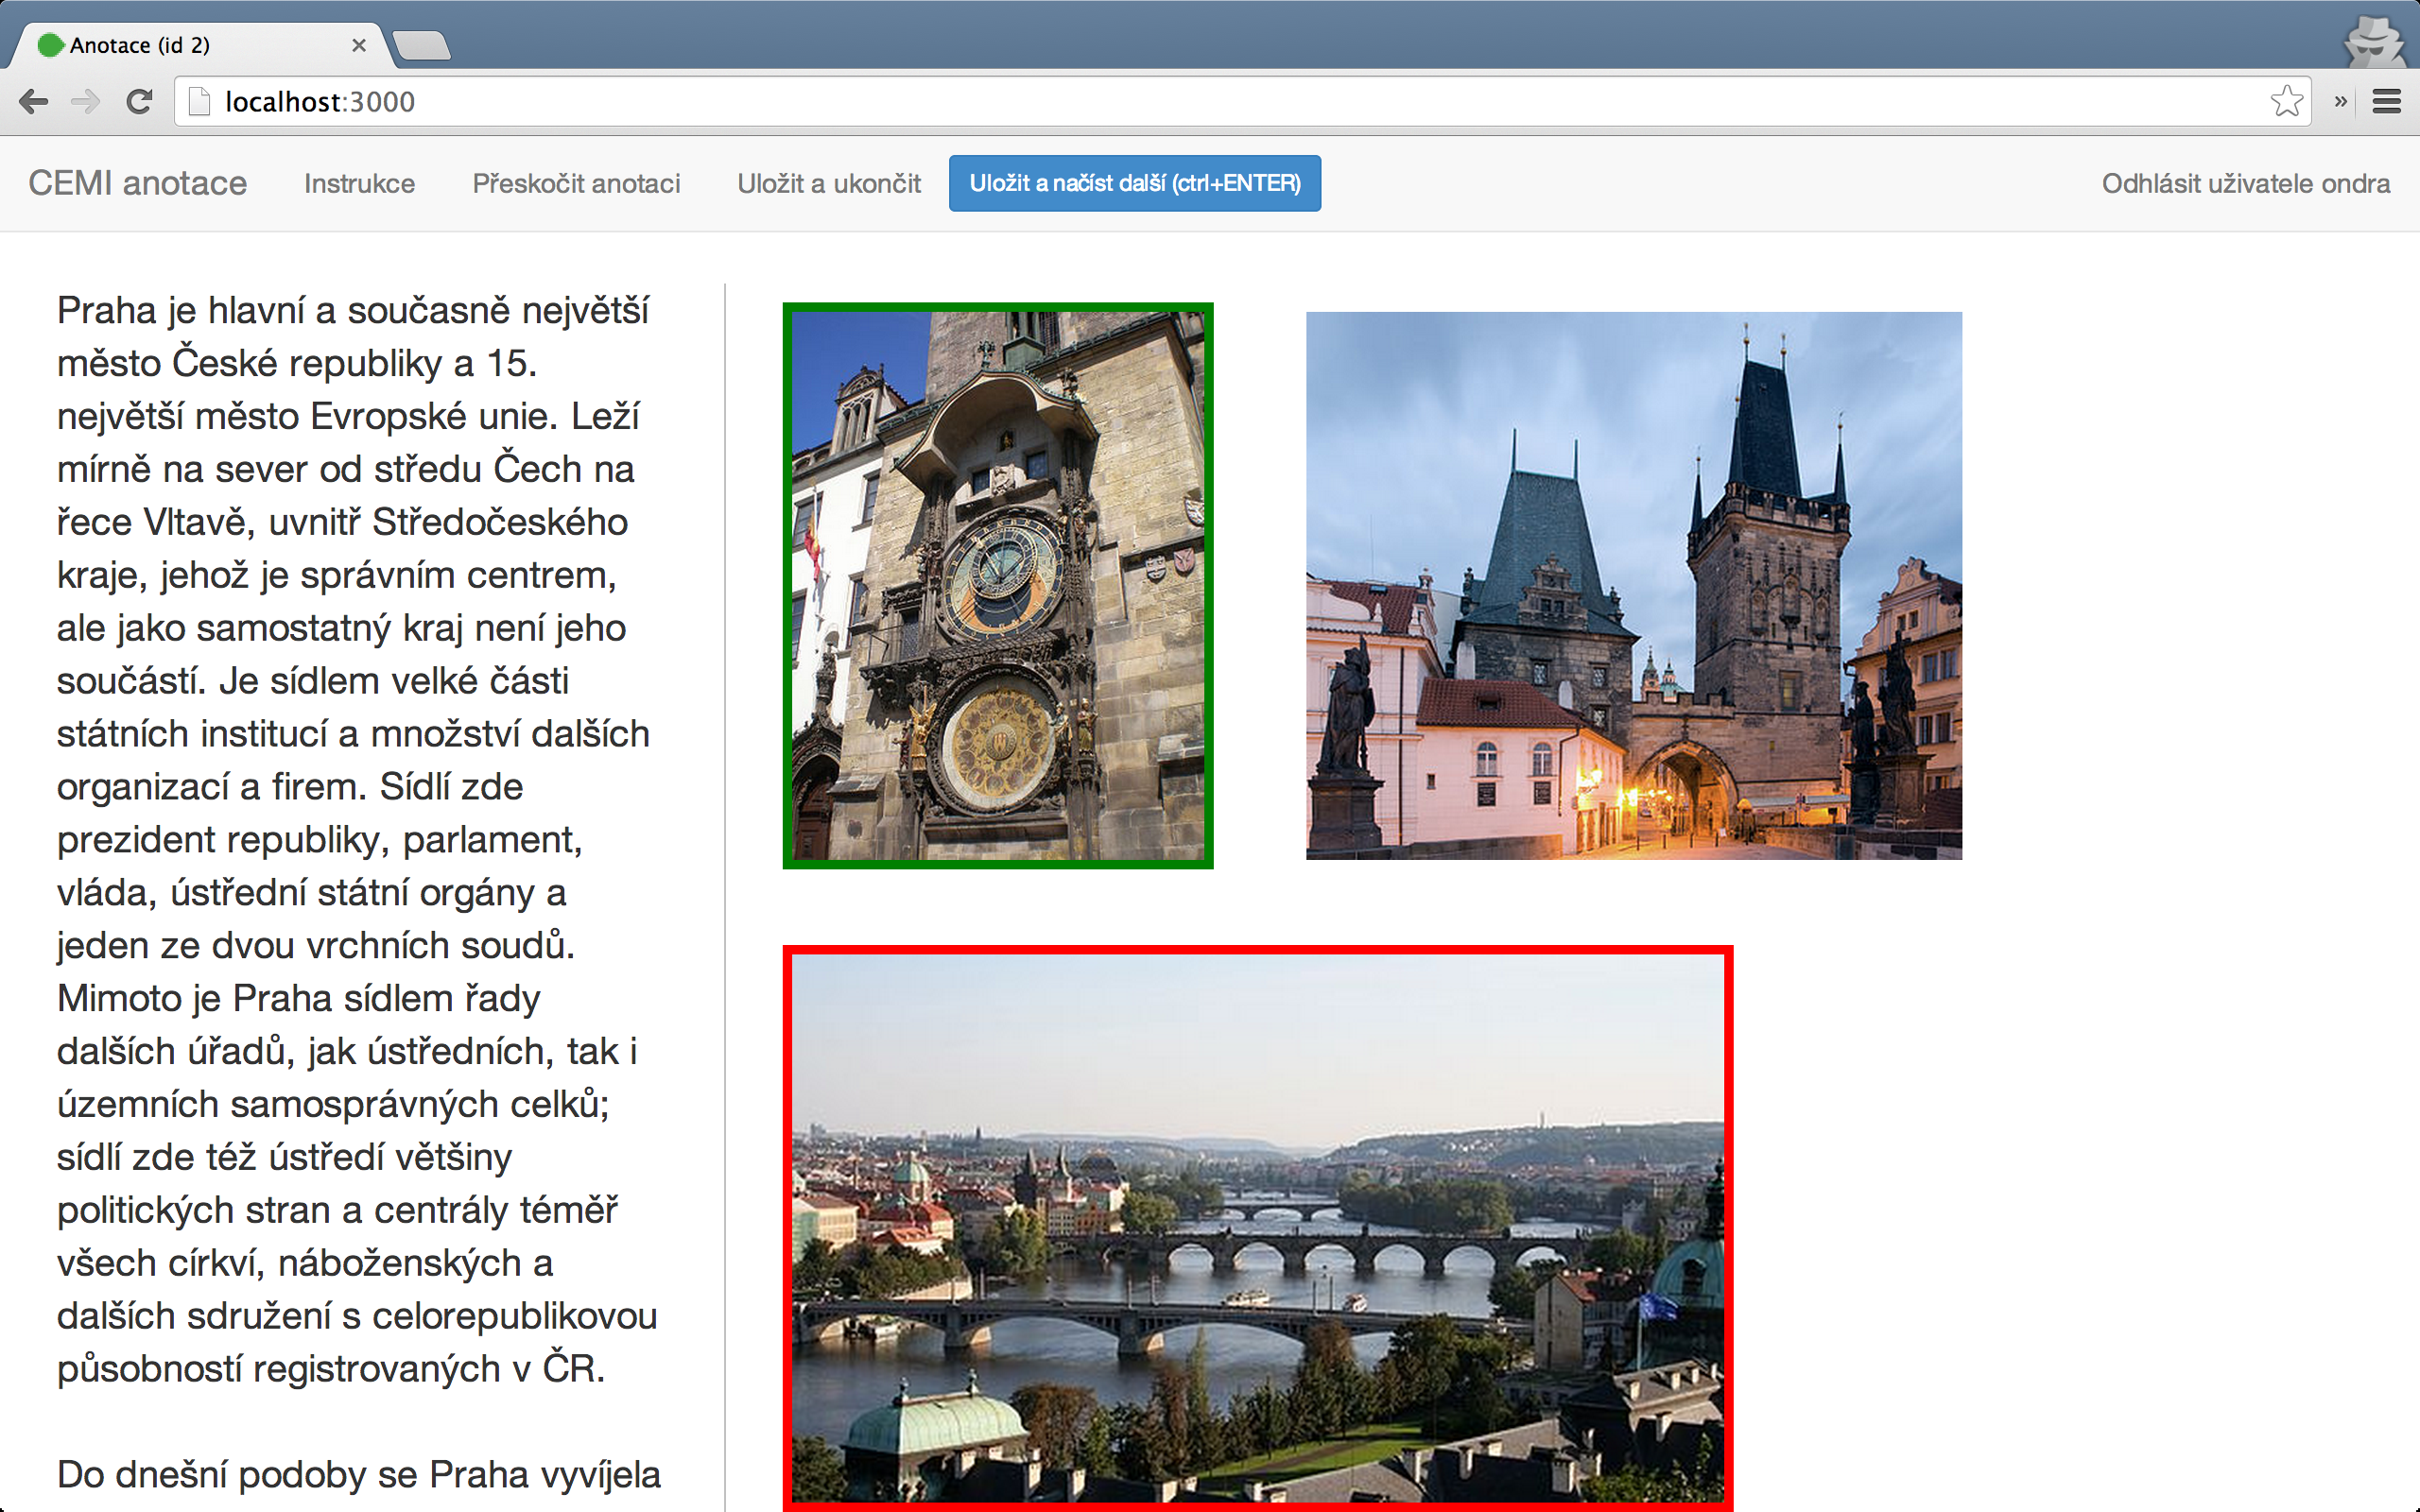
\includegraphics[width=150mm]{anotacni_rozhrani.eps}
  \caption{Anotační rozhraní. Vhodné obrázky jsou označené zeleným rámečkem, nevhodné červeným.}
  \label{fig:anotacni_rozhrani}
\end{figure}

\section{Anotační proces}

Úkolem anotátora je přiřadit vhodné a nevhodné obrázky. Po přihlášení do~anotačního rozhraní vidí v~levé části test a v~pravé obrázky. Levým tlačítkem myši může označit obrázky, které odpovídají textu, pravým tlačítkem myši označí obrázky, které textu neodpovídají. Pokud si anotátor není jistý, nechá obrázek neoznačený. Uživatel může použít klávesovou zkratku \uv{ctrl+ENTER} k~uložení a načtení další anotace. Může také anotaci přeskočit (pak se označí jako přeskočená a nepřiřadí se jinému anotátorovi), nebo uložit a ukončit.



